\begin{quote}
This is part of Categories for Programmers. Previously:
\href{https://bartoszmilewski.com/2015/01/13/simple-algebraic-data-types/}{Simple
Algebraic Data Types}. See the
\href{https://bartoszmilewski.com/2014/10/28/category-theory-for-programmers-the-preface/}{Table
of Contents}.
\end{quote}

At the risk of sounding like a broken record, I will say this about
functors: A functor is a very simple but powerful idea. Category theory
is just full of those simple but powerful ideas. A functor is a mapping
between categories. Given two categories, C and D, a functor F maps
objects in C to objects in D --- it's a function on objects. If \emph{a}
is an object in C, we'll write its image in D as \emph{F a} (no
parentheses). But a category is not just objects --- it's objects and
morphisms that connect them. A functor also maps morphisms --- it's a
function on morphisms. But it doesn't map morphisms willy-nilly --- it
preserves connections. So if a morphism \emph{f} in C connects object
\emph{a} to object \emph{b},

\begin{verbatim}
f :: a -> b
\end{verbatim}

the image of \emph{f} in D, \emph{F f}, will connect the image of
\emph{a} to the image of \emph{b}:

\begin{verbatim}
F f :: F a -> F b
\end{verbatim}

(This is a mixture of mathematical and Haskell notation that hopefully
makes sense by now. I won't use parentheses when applying functors to
objects or morphisms.)
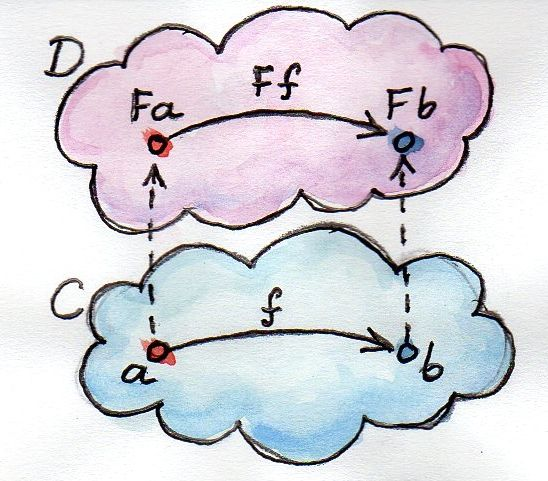
\includegraphics[width=3.12500in]{images/functor.jpg} As you can see, a
functor preserves the structure of a category: what's connected in one
category will be connected in the other category. But there's something
more to the structure of a category: there's also the composition of
morphisms. If \emph{h} is a composition of \emph{f} and \emph{g}:

\begin{verbatim}
h = g . f
\end{verbatim}

we want its image under F to be a composition of the images of \emph{f}
and \emph{g}:

\begin{verbatim}
F h = F g . F f
\end{verbatim}

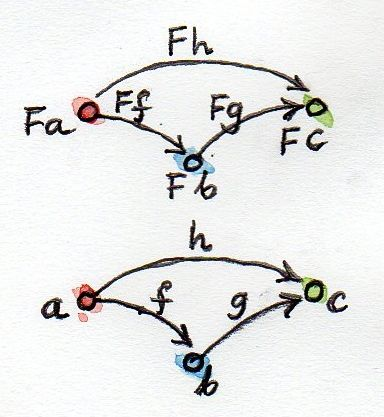
\includegraphics[width=2.87500in]{images/functorcompos.jpg} Finally, we
want all identity morphisms in C to be mapped to identity morphisms in
D:

\begin{verbatim}
F ida = idF a
\end{verbatim}

Here, \emph{id\textsubscript{a}} is the identity at the object \emph{a},
and \emph{id\textsubscript{F a}} the identity at \emph{F a}.
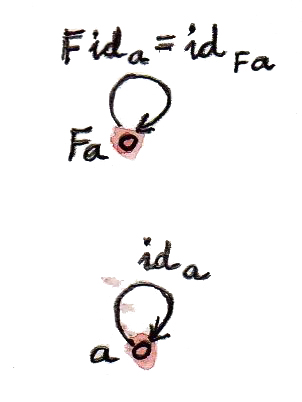
\includegraphics[width=2.34375in]{images/functorid.jpg} Note that these
conditions make functors much more restrictive than regular functions.
Functors must preserve the structure of a category. If you picture a
category as a collection of objects held together by a network of
morphisms, a functor is not allowed to introduce any tears into this
fabric. It may smash objects together, it may glue multiple morphisms
into one, but it may never break things apart. This no-tearing
constraint is similar to the continuity condition you might know from
calculus. In this sense functors are ``continuous'' (although there
exists an even more restrictive notion of continuity for functors). Just
like functions, functors may do both collapsing and embedding. The
embedding aspect is more prominent when the source category is much
smaller than the target category. In the extreme, the source can be the
trivial singleton category --- a category with one object and one
morphism (the identity). A functor from the singleton category to any
other category simply selects an object in that category. This is fully
analogous to the property of morphisms from singleton sets selecting
elements in target sets. The maximally collapsing functor is called the
constant functor Δ\textsubscript{c}. It maps every object in the source
category to one selected object \emph{c} in the target category. It also
maps every morphism in the source category to the identity morphism
\emph{id\textsubscript{c}}. It acts like a black hole, compacting
everything into one singularity. We'll see more of this functor when we
discuss limits and colimits.

\subsection{Functors in Programming}\label{functors-in-programming}

Let's get down to earth and talk about programming. We have our category
of types and functions. We can talk about functors that map this
category into itself --- such functors are called endofunctors. So
what's an endofunctor in the category of types? First of all, it maps
types to types. We've seen examples of such mappings, maybe without
realizing that they were just that. I'm talking about definitions of
types that were parameterized by other types. Let's see a few examples.

\subsubsection{The Maybe Functor}\label{the-maybe-functor}

The definition of \texttt{Maybe} is a mapping from type \texttt{a} to
type \texttt{Maybe\ a}:

\begin{verbatim}
data Maybe a = Nothing | Just a
\end{verbatim}

Here's an important subtlety: \texttt{Maybe} itself is not a type, it's
a \emph{type constructor}. You have to give it a type argument, like
\texttt{Int} or \texttt{Bool}, in order to turn it into a type.
\texttt{Maybe} without any argument represents a function on types. But
can we turn \texttt{Maybe} into a functor? (From now on, when I speak of
functors in the context of programming, I will almost always mean
endofunctors.) A functor is not only a mapping of objects (here, types)
but also a mapping of morphisms (here, functions). For any function from
\texttt{a} to \texttt{b}:

\begin{verbatim}
f :: a -> b
\end{verbatim}

we would like to produce a function from \texttt{Maybe\ a} to
\texttt{Maybe\ b}. To define such a function, we'll have two cases to
consider, corresponding to the two constructors of \texttt{Maybe}. The
\texttt{Nothing} case is simple: we'll just return \texttt{Nothing}
back. And if the argument is \texttt{Just}, we'll apply the function
\texttt{f} to its contents. So the image of \texttt{f} under
\texttt{Maybe} is the function:

\begin{verbatim}
f’ :: Maybe a -> Maybe b f’ Nothing = Nothing f’ (Just x) = Just (f x)
\end{verbatim}

(By the way, in Haskell you can use apostrophes in variables names,
which is very handy in cases like these.) In Haskell, we implement the
morphism-mapping part of a functor as a higher order function called
\texttt{fmap}. In the case of \texttt{Maybe}, it has the following
signature:

\begin{verbatim}
fmap :: (a -> b) -> (Maybe a -> Maybe b)
\end{verbatim}

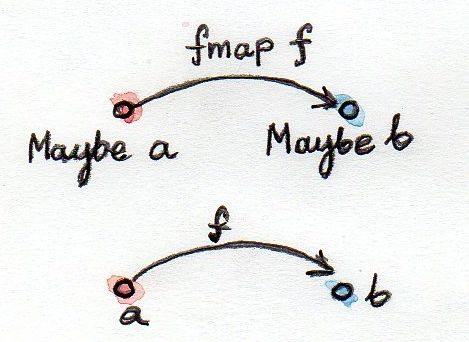
\includegraphics[width=3.12500in]{images/functormaybe.jpg} We often say
that \texttt{fmap} \emph{lifts} a function. The lifted function acts on
\texttt{Maybe} values. As usual, because of currying, this signature may
be interpreted in two ways: as a function of one argument --- which
itself is a function \texttt{(a-\textgreater{}b)} --- returning a
function \texttt{(Maybe\ a\ -\textgreater{}\ Maybe\ b)}; or as a
function of two arguments returning \texttt{Maybe\ b}:

\begin{verbatim}
fmap :: (a -> b) -> Maybe a -> Maybe b
\end{verbatim}

Based on our previous discussion, this is how we implement \texttt{fmap}
for \texttt{Maybe}:

\begin{verbatim}
fmap _ Nothing = Nothing fmap f (Just x) = Just (f x)
\end{verbatim}

To show that the type constructor \texttt{Maybe} together with the
function \texttt{fmap} form a functor, we have to prove that
\texttt{fmap} preserves identity and composition. These are called ``the
functor laws,'' but they simply ensure the preservation of the structure
of the category.

\subsubsection{Equational Reasoning}\label{equational-reasoning}

To prove the functor laws, I will use \emph{equational reasoning}, which
is a common proof technique in Haskell. It takes advantage of the fact
that Haskell functions are defined as equalities: the left hand side
equals the right hand side. You can always substitute one for another,
possibly renaming variables to avoid name conflicts. Think of this as
either inlining a function, or the other way around, refactoring an
expression into a function. Let's take the identity function as an
example:

\begin{verbatim}
id x = x
\end{verbatim}

If you see, for instance, \texttt{id\ y} in some expression, you can
replace it with \texttt{y} (inlining). Further, if you see \texttt{id}
applied to an expression, say \texttt{id\ (y\ +\ 2)}, you can replace it
with the expression itself \texttt{(y\ +\ 2)}. And this substitution
works both ways: you can replace any expression \texttt{e} with
\texttt{id\ e} (refactoring). If a function is defined by pattern
matching, you can use each sub-definition independently. For instance,
given the above definition of \texttt{fmap} you can replace
\texttt{fmap\ f\ Nothing} with \texttt{Nothing}, or the other way
around. Let's see how this works in practice. Let's start with the
preservation of identity:

\begin{verbatim}
fmap id = id
\end{verbatim}

There are two cases to consider: \texttt{Nothing} and \texttt{Just}.
Here's the first case (I'm using Haskell pseudo-code to transform the
left hand side to the right hand side):

\begin{verbatim}
 fmap id Nothing = { definition of fmap } Nothing = { definition of id } id Nothing
\end{verbatim}

Notice that in the last step I used the definition of \texttt{id}
backwards. I replaced the expression \texttt{Nothing} with
\texttt{id\ Nothing}. In practice, you carry out such proofs by
``burning the candle at both ends,'' until you hit the same expression
in the middle --- here it was \texttt{Nothing}. The second case is also
easy:

\begin{verbatim}
 fmap id (Just x) = { definition of fmap } Just (id x) = { definition of id } Just x = { definition of id } id (Just x)
\end{verbatim}

Now, lets show that \texttt{fmap} preserves composition:

\begin{verbatim}
fmap (g . f) = fmap g . fmap f
\end{verbatim}

First the \texttt{Nothing} case:

\begin{verbatim}
 fmap (g . f) Nothing = { definition of fmap } Nothing = { definition of fmap } fmap g Nothing = { definition of fmap } fmap g (fmap f Nothing)
\end{verbatim}

And then the \texttt{Just} case:

\begin{verbatim}
 fmap (g . f) (Just x) = { definition of fmap } Just ((g . f) x) = { definition of composition } Just (g (f x)) = { definition of fmap } fmap g (Just (f x)) = { definition of fmap } fmap g (fmap f (Just x)) = { definition of composition } (fmap g . fmap f) (Just x)
\end{verbatim}

It's worth stressing that equational reasoning doesn't work for C++
style ``functions'' with side effects. Consider this code:

\begin{verbatim}
int square(int x) { return x * x; } int counter() { static int c = 0; return c++; } double y = square(counter());
\end{verbatim}

Using equational reasoning, you would be able to inline \texttt{square}
to get:

\begin{verbatim}
double y = counter() * counter();
\end{verbatim}

This is definitely not a valid transformation, and it will not produce
the same result. Despite that, the C++ compiler will try to use
equational reasoning if you implement \texttt{square} as a macro, with
disastrous results.

\subsubsection{Optional}\label{optional}

Functors are easily expressed in Haskell, but they can be defined in any
language that supports generic programming and higher-order functions.
Let's consider the C++ analog of \texttt{Maybe}, the template type
\texttt{optional}. Here's a sketch of the implementation (the actual
implementation is much more complex, dealing with various ways the
argument may be passed, with copy semantics, and with the resource
management issues characteristic of C++):

\begin{verbatim}
template<class T> class optional { bool _isValid; // the tag T _v; public: optional() : _isValid(false) {} // Nothing optional(T x) : _isValid(true) , _v(x) {} // Just bool isValid() const { return _isValid; } T val() const { return _v; } };
\end{verbatim}

This template provides one part of the definition of a functor: the
mapping of types. It maps any type \texttt{T} to a new type
\texttt{optional\textless{}T\textgreater{}}. Let's define its action on
functions:

\begin{verbatim}
template<class A, class B> std::function<optional<B>(optional<A>)> fmap(std::function<B(A)> f) { return [f](optional<A> opt) { if (!opt.isValid()) return optional<B>{}; else return optional<B>{ f(opt.val()) }; }; }
\end{verbatim}

This is a higher order function, taking a function as an argument and
returning a function. Here's the uncurried version of it:

\begin{verbatim}
template<class A, class B> optional<B> fmap(std::function<B(A)> f, optional<A> opt) { if (!opt.isValid()) return optional<B>{}; else return optional<B>{ f(opt.val()) }; }
\end{verbatim}

There is also an option of making \texttt{fmap} a template method of
\texttt{optional}. This embarrassment of choices makes abstracting the
functor pattern in C++ a problem. Should functor be an interface to
inherit from (unfortunately, you can't have template virtual functions)?
Should it be a curried or an uncurried free template function? Can the
C++ compiler correctly infer the missing types, or should they be
specified explicitly? Consider a situation where the input function
\texttt{f} takes an \texttt{int} to a \texttt{bool}. How will the
compiler figure out the type of \texttt{g}:

\begin{verbatim}
auto g = fmap(f);
\end{verbatim}

especially if, in the future, there are multiple functors overloading
\texttt{fmap}? (We'll see more functors soon.)

\subsubsection{Typeclasses}\label{typeclasses}

So how does Haskell deal with abstracting the functor? It uses the
typeclass mechanism. A typeclass defines a family of types that support
a common interface. For instance, the class of objects that support
equality is defined as follows:

\begin{verbatim}
class Eq a where (==) :: a -> a -> Bool
\end{verbatim}

This definition states that type \texttt{a} is of the class \texttt{Eq}
if it supports the operator \texttt{(==)} that takes two arguments of
type \texttt{a} and returns a \texttt{Bool}. If you want to tell Haskell
that a particular type is \texttt{Eq}, you have to declare it an
\emph{instance} of this class and provide the implementation of
\texttt{(==)}. For example, given the definition of a 2D \texttt{Point}
(a product type of two \texttt{Float}s):

\begin{verbatim}
data Point = Pt Float Float
\end{verbatim}

you can define the equality of points:

\begin{verbatim}
instance Eq Point where (Pt x y) == (Pt x&apos; y&apos;) = x == x&apos; && y == y&apos;
\end{verbatim}

Here I used the operator \texttt{(==)} (the one I'm defining) in the
infix position between the two patterns \texttt{(Pt\ x\ y)} and
\texttt{(Pt\ x\&apos;\ y\&apos;)}. The body of the function follows the
single equal sign. Once \texttt{Point} is declared an instance of
\texttt{Eq}, you can directly compare points for equality. Notice that,
unlike in C++ or Java, you don't have to specify the \texttt{Eq} class
(or interface) when defining \texttt{Point} --- you can do it later in
client code. Typeclasses are also Haskell's only mechanism for
overloading functions (and operators). We will need that for overloading
\texttt{fmap} for different functors. There is one complication, though:
a functor is not defined as a type but as a mapping of types, a type
constructor. We need a typeclass that's not a family of types, as was
the case with \texttt{Eq}, but a family of type constructors.
Fortunately a Haskell typeclass works with type constructors as well as
with types. So here's the definition of the \texttt{Functor} class:

\begin{verbatim}
class Functor f where fmap :: (a -> b) -> f a -> f b
\end{verbatim}

It stipulates that \texttt{f} is a \texttt{Functor} if there exists a
function \texttt{fmap} with the specified type signature. The lowercase
\texttt{f} is a type variable, similar to type variables \texttt{a} and
\texttt{b}. The compiler, however, is able to deduce that it represents
a type constructor rather than a type by looking at its usage: acting on
other types, as in \texttt{f\ a} and \texttt{f\ b}. Accordingly, when
declaring an instance of \texttt{Functor}, you have to give it a type
constructor, as is the case with \texttt{Maybe}:

\begin{verbatim}
instance Functor Maybe where fmap _ Nothing = Nothing fmap f (Just x) = Just (f x)
\end{verbatim}

By the way, the \texttt{Functor} class, as well as its instance
definitions for a lot of simple data types, including \texttt{Maybe},
are part of the standard Prelude library.

\subsubsection{Functor in C++}\label{functor-in-c}

Can we try the same approach in C++? A type constructor corresponds to a
template class, like \texttt{optional}, so by analogy, we would
parameterize \texttt{fmap} with a \emph{template template parameter}
\texttt{F}. This is the syntax for it:

\begin{verbatim}
template<template<class> F, class A, class B> F<B> fmap(std::function<B(A)>, F<A>);
\end{verbatim}

We would like to be able to specialize this template for different
functors. Unfortunately, there is a prohibition against partial
specialization of template functions in C++. You can't write:

\begin{verbatim}
template<class A, class B> optional<B> fmap<optional>(std::function<B(A)> f, optional<A> opt)
\end{verbatim}

Instead, we have to fall back on function overloading, which brings us
back to the original definition of the uncurried \texttt{fmap}:

\begin{verbatim}
template<class A, class B> optional<B> fmap(std::function<B(A)> f, optional<A> opt) { if (!opt.isValid()) return optional<B>{}; else return optional<B>{ f(opt.val()) }; }
\end{verbatim}

This definition works, but only because the second argument of
\texttt{fmap} selects the overload. It totally ignores the more generic
definition of \texttt{fmap}.

\subsubsection{The List Functor}\label{the-list-functor}

To get some intuition as to the role of functors in programming, we need
to look at more examples. Any type that is parameterized by another type
is a candidate for a functor. Generic containers are parameterized by
the type of the elements they store, so let's look at a very simple
container, the list:

\begin{verbatim}
data List a = Nil | Cons a (List a)
\end{verbatim}

We have the type constructor \texttt{List}, which is a mapping from any
type \texttt{a} to the type \texttt{List\ a}. To show that \texttt{List}
is a functor we have to define the lifting of functions: Given a
function \texttt{a-\textgreater{}b} define a function
\texttt{List\ a\ -\textgreater{}\ List\ b}:

\begin{verbatim}
fmap :: (a -> b) -> (List a -> List b)
\end{verbatim}

A function acting on \texttt{List\ a} must consider two cases
corresponding to the two list constructors. The \texttt{Nil} case is
trivial --- just return \texttt{Nil} --- there isn't much you can do
with an empty list. The \texttt{Cons} case is a bit tricky, because it
involves recursion. So let's step back for a moment and consider what we
are trying to do. We have a list of \texttt{a}, a function \texttt{f}
that turns \texttt{a} to \texttt{b}, and we want to generate a list of
\texttt{b}. The obvious thing is to use \texttt{f} to turn each element
of the list from \texttt{a} to \texttt{b}. How do we do this in
practice, given that a (non-empty) list is defined as the \texttt{Cons}
of a head and a tail? We apply \texttt{f} to the head and apply the
lifted (\texttt{fmap}ped) \texttt{f} to the tail. This is a recursive
definition, because we are defining lifted \texttt{f} in terms of lifted
\texttt{f}:

\begin{verbatim}
fmap f (Cons x t) = Cons (f x) (fmap f t)
\end{verbatim}

Notice that, on the right hand side, \texttt{fmap\ f} is applied to a
list that's shorter than the list for which we are defining it --- it's
applied to its tail. We recurse towards shorter and shorter lists, so we
are bound to eventually reach the empty list, or \texttt{Nil}. But as
we've decided earlier, \texttt{fmap\ f} acting on \texttt{Nil} returns
\texttt{Nil}, thus terminating the recursion. To get the final result,
we combine the new head \texttt{(f\ x)} with the new tail
\texttt{(fmap\ f\ t)} using the \texttt{Cons} constructor. Putting it
all together, here's the instance declaration for the list functor:

\begin{verbatim}
instance Functor List where fmap _ Nil = Nil fmap f (Cons x t) = Cons (f x) (fmap f t)
\end{verbatim}

If you are more comfortable with C++, consider the case of a
\texttt{std::vector}, which could be considered the most generic C++
container. The implementation of \texttt{fmap} for \texttt{std::vector}
is just a thin encapsulation of \texttt{std::transform}:

\begin{verbatim}
template<class A, class B> std::vector<B> fmap(std::function<B(A)> f, std::vector<A> v) { std::vector<B> w; std::transform( std::begin(v) , std::end(v) , std::back_inserter(w) , f); return w; }
\end{verbatim}

We can use it, for instance, to square the elements of a sequence of
numbers:

\begin{verbatim}
std::vector<int> v{ 1, 2, 3, 4 }; auto w = fmap([](int i) { return i*i; }, v); std::copy( std::begin(w) , std::end(w) , std::ostream_iterator(std::cout, ", "));
\end{verbatim}

Most C++ containers are functors by virtue of implementing iterators
that can be passed to \texttt{std::transform}, which is the more
primitive cousin of \texttt{fmap}. Unfortunately, the simplicity of a
functor is lost under the usual clutter of iterators and temporaries
(see the implementation of \texttt{fmap} above). I'm happy to say that
the new proposed C++ range library makes the functorial nature of ranges
much more pronounced.

\subsubsection{The Reader Functor}\label{the-reader-functor}

Now that you might have developed some intuitions --- for instance,
functors being some kind of containers --- let me show you an example
which at first sight looks very different. Consider a mapping of type
\texttt{a} to the type of a function returning \texttt{a}. We haven't
really talked about function types in depth --- the full categorical
treatment is coming --- but we have some understanding of those as
programmers. In Haskell, a function type is constructed using the arrow
type constructor \texttt{(-\textgreater{})} which takes two types: the
argument type and the result type. You've already seen it in infix form,
\texttt{a-\textgreater{}b}, but it can equally well be used in prefix
form, when parenthesized:

\begin{verbatim}
(->) a b
\end{verbatim}

Just like with regular functions, type functions of more than one
argument can be partially applied. So when we provide just one type
argument to the arrow, it still expects another one. That's why:

\begin{verbatim}
(->) a
\end{verbatim}

is a type constructor. It needs one more type \texttt{b} to produce a
complete type \texttt{a-\textgreater{}b}. As it stands, it defines a
whole family of type constructors parameterized by \texttt{a}. Let's see
if this is also a family of functors. Dealing with two type parameters
can get a bit confusing, so let's do some renaming. Let's call the
argument type \texttt{r} and the result type \texttt{a}, in line with
our previous functor definitions. So our type constructor takes any type
\texttt{a} and maps it into the type \texttt{r-\textgreater{}a}. To show
that it's a functor, we want to lift a function
\texttt{a-\textgreater{}b} to a function that takes
\texttt{r-\textgreater{}a} and returns \texttt{r-\textgreater{}b}. These
are the types that are formed using the type constructor
\texttt{(-\textgreater{})\ r} acting on, respectively, \texttt{a} and
\texttt{b}. Here's the type signature of \texttt{fmap} applied to this
case:

\begin{verbatim}
fmap :: (a -> b) -> (r -> a) -> (r -> b)
\end{verbatim}

We have to solve the following puzzle: given a function
\texttt{f::a-\textgreater{}b} and a function
\texttt{g::r-\textgreater{}a}, create a function
\texttt{r-\textgreater{}b}. There is only one way we can compose the two
functions, and the result is exactly what we need. So here's the
implementation of our \texttt{fmap}:

\begin{verbatim}
instance Functor ((->) r) where fmap f g = f . g
\end{verbatim}

It just works! If you like terse notation, this definition can be
reduced further by noticing that composition can be rewritten in prefix
form:

\begin{verbatim}
fmap f g = (.) f g
\end{verbatim}

and the arguments can be omitted to yield a direct equality of two
functions:

\begin{verbatim}
fmap = (.)
\end{verbatim}

This combination of the type constructor \texttt{(-\textgreater{})\ r}
with the above implementation of \texttt{fmap} is called the reader
functor.

\subsection{Functors as Containers}\label{functors-as-containers}

We've seen some examples of functors in programming languages that
define general-purpose containers, or at least objects that contain some
value of the type they are parameterized over. The reader functor seems
to be an outlier, because we don't think of functions as data. But we've
seen that pure functions can be memoized, and function execution can be
turned into table lookup. Tables are data. Conversely, because of
Haskell's laziness, a traditional container, like a list, may actually
be implemented as a function. Consider, for instance, an infinite list
of natural numbers, which can be compactly defined as:

\begin{verbatim}
nats :: [Integer] nats = [1..]
\end{verbatim}

In the first line, a pair of square brackets is Haskell's built-in type
constructor for lists. In the second line, square brackets are used to
create a list literal. Obviously, an infinite list like this cannot be
stored in memory. The compiler implements it as a function that
generates \texttt{Integer}s on demand. Haskell effectively blurs the
distinction between data and code. A list could be considered a
function, and a function could be considered a table that maps arguments
to results. The latter can even be practical if the domain of the
function is finite and not too large. It would not be practical,
however, to implement \texttt{strlen} as table lookup, because there are
infinitely many different strings. As programmers, we don't like
infinities, but in category theory you learn to eat infinities for
breakfast. Whether it's a set of all strings or a collection of all
possible states of the Universe, past, present, and future --- we can
deal with it! So I like to think of the functor object (an object of the
type generated by an endofunctor) as containing a value or values of the
type over which it is parameterized, even if these values are not
physically present there. One example of a functor is a C++
\texttt{std::future}, which may at some point contain a value, but it's
not guaranteed it will; and if you want to access it, you may block
waiting for another thread to finish execution. Another example is a
Haskell \texttt{IO} object, which may contain user input, or the future
versions of our Universe with ``Hello World!'' displayed on the monitor.
According to this interpretation, a functor object is something that may
contain a value or values of the type it's parameterized upon. Or it may
contain a recipe for generating those values. We are not at all
concerned about being able to access the values --- that's totally
optional, and outside of the scope of the functor. All we are interested
in is to be able to manipulate those values using functions. If the
values can be accessed, then we should be able to see the results of
this manipulation. If they can't, then all we care about is that the
manipulations compose correctly and that the manipulation with an
identity function doesn't change anything. Just to show you how much we
don't care about being able to access the values inside a functor
object, here's a type constructor that ignores completely its argument
\texttt{a}:

\begin{verbatim}
data Const c a = Const c
\end{verbatim}

The \texttt{Const} type constructor takes two types, \texttt{c} and
\texttt{a}. Just like we did with the arrow constructor, we are going to
partially apply it to create a functor. The data constructor (also
called \texttt{Const}) takes just one value of type \texttt{c}. It has
no dependence on \texttt{a}. The type of \texttt{fmap} for this type
constructor is:

\begin{verbatim}
fmap :: (a -> b) -> Const c a -> Const c b
\end{verbatim}

Because the functor ignores its type argument, the implementation of
\texttt{fmap} is free to ignore its function argument --- the function
has nothing to act upon:

\begin{verbatim}
instance Functor (Const c) where fmap _ (Const v) = Const v
\end{verbatim}

This might be a little clearer in C++ (I never thought I would utter
those words!), where there is a stronger distinction between type
arguments --- which are compile-time --- and values, which are run-time:

\begin{verbatim}
template<class C, class A> struct Const { Const(C v) : _v(v) {} C _v; };
\end{verbatim}

The C++ implementation of \texttt{fmap} also ignores the function
argument and essentially re-casts the \texttt{Const} argument without
changing its value:

\begin{verbatim}
template<class C, class A, class B> Const<C, B> fmap(std::function<B(A)> f, Const<C, A> c) { return Const<C, B>{c._v}; }
\end{verbatim}

Despite its weirdness, the \texttt{Const} functor plays an important
role in many constructions. In category theory, it's a special case of
the Δ\textsubscript{c} functor I mentioned earlier --- the endo-functor
case of a black hole. We'll be seeing more of it it in the future.

\subsection{Functor Composition}\label{functor-composition}

It's not hard to convince yourself that functors between categories
compose, just like functions between sets compose. A composition of two
functors, when acting on objects, is just the composition of their
respective object mappings; and similarly when acting on morphisms.
After jumping through two functors, identity morphisms end up as
identity morphisms, and compositions of morphisms finish up as
compositions of morphisms. There's really nothing much to it. In
particular, it's easy to compose endofunctors. Remember the function
\texttt{maybeTail}? I'll rewrite it using Haskell's built in
implementation of lists:

\begin{verbatim}
maybeTail :: [a] -> Maybe [a] maybeTail [] = Nothing maybeTail (x:xs) = Just xs
\end{verbatim}

(The empty list constructor that we used to call \texttt{Nil} is
replaced with the empty pair of square brackets \texttt{{[}{]}}. The
\texttt{Cons} constructor is replaced with the infix operator \texttt{:}
(colon).) The result of \texttt{maybeTail} is of a type that's a
composition of two functors, \texttt{Maybe} and \texttt{{[}{]}}, acting
on \texttt{a}. Each of these functors is equipped with its own version
of \texttt{fmap}, but what if we want to apply some function \texttt{f}
to the contents of the composite: a \texttt{Maybe} list? We have to
break through two layers of functors. We can use \texttt{fmap} to break
through the outer \texttt{Maybe}. But we can't just send \texttt{f}
inside \texttt{Maybe} because \texttt{f} doesn't work on lists. We have
to send \texttt{(fmap\ f)} to operate on the inner list. For instance,
let's see how we can square the elements of a \texttt{Maybe} list of
integers:

\begin{verbatim}
square x = x * x mis :: Maybe [Int] mis = Just [1, 2, 3] mis2 = fmap (fmap square) mis
\end{verbatim}

The compiler, after analyzing the types, will figure out that, for the
outer \texttt{fmap}, it should use the implementation from the
\texttt{Maybe} instance, and for the inner one, the list functor
implementation. It may not be immediately obvious that the above code
may be rewritten as:

\begin{verbatim}
mis2 = (fmap . fmap) square mis
\end{verbatim}

But remember that \texttt{fmap} may be considered a function of just one
argument:

\begin{verbatim}
fmap :: (a -> b) -> (f a -> f b)
\end{verbatim}

In our case, the second \texttt{fmap} in \texttt{(fmap\ .\ fmap)} takes
as its argument:

\begin{verbatim}
square :: Int -> Int
\end{verbatim}

and returns a function of the type:

\begin{verbatim}
[Int] -> [Int]
\end{verbatim}

The first \texttt{fmap} then takes that function and returns a function:

\begin{verbatim}
Maybe [Int] -> Maybe [Int]
\end{verbatim}

Finally, that function is applied to \texttt{mis}. So the composition of
two functors is a functor whose \texttt{fmap} is the composition of the
corresponding \texttt{fmap}s. Going back to category theory: It's pretty
obvious that functor composition is associative (the mapping of objects
is associative, and the mapping of morphisms is associative). And there
is also a trivial identity functor in every category: it maps every
object to itself, and every morphism to itself. So functors have all the
same properties as morphisms in some category. But what category would
that be? It would have to be a category in which objects are categories
and morphisms are functors. It's a category of categories. But a
category of \emph{all} categories would have to include itself, and we
would get into the same kinds of paradoxes that made the set of all sets
impossible. There is, however, a category of all \emph{small} categories
called \textbf{Cat} (which is big, so it can't be a member of itself). A
small category is one in which objects form a set, as opposed to
something larger than a set. Mind you, in category theory, even an
infinite uncountable set is considered ``small.'' I thought I'd mention
these things because I find it pretty amazing that we can recognize the
same structures repeating themselves at many levels of abstraction.
We'll see later that functors form categories as well.

\subsection{Challenges}\label{challenges}

\begin{enumerate}
\item
  Can we turn the \texttt{Maybe} type constructor into a functor by
  defining:

\begin{verbatim}
fmap _ _ = Nothing
\end{verbatim}

  which ignores both of its arguments? (Hint: Check the functor laws.)
\item
  Prove functor laws for the reader functor. Hint: it's really simple.
\item
  Implement the reader functor in your second favorite language (the
  first being Haskell, of course).
\item
  Prove the functor laws for the list functor. Assume that the laws are
  true for the tail part of the list you're applying it to (in other
  words, use \emph{induction}).
\end{enumerate}

\subsection{Acknowledgments}\label{acknowledgments}

Gershom Bazerman is kind enough to keep reviewing these posts. I'm
grateful for his patience and insight.

\emph{Next:
\href{https://bartoszmilewski.com/2015/02/03/functoriality/}{Functoriality}}

\href{https://twitter.com/BartoszMilewski}{Follow @BartoszMilewski}
